\documentclass[a4paper]{article}
\usepackage{amsmath}
\usepackage{graphicx}
\usepackage{geometry}
\usepackage{floatrow}
\usepackage{layout}
\usepackage{amssymb} 
\usepackage{multirow}
\usepackage{caption}
\geometry{margin=1in}
\usepackage{authblk}
\usepackage{indentfirst}
\usepackage[hidelinks]{hyperref}

\providecommand{\keywords}[1]
{
  \small	
  \textbf{\; \textit{Keywords---}} #1
}

\begin{document}

\title{\textbf{\huge{Insert Fancy Project Title}}}

\author{\textbf\large{Author 1, Author 2, Author 3}}


\affil{\textbf{XYZ University, City, ZIP code}}

\date{\today}

\maketitle
\begin{abstract}
Your abstract goes here. A well-written abstract introduces the problem and motivation (briefly), highlights the approach taken by the authors, and summarizes the results. The idea is to give the readers an overview of what to expect from the paper.
\end{abstract}\maketitle

\keywords{\textbf{one}, \textbf{two}, \textbf{three} \\(Example: \textbf{Community Detection}, \textbf{Biological Network Analysis}, \textbf{Efficiency Comparison})}

\section*{Introduction}

The introduction section serves to expand upon the motivation, and to contextualize the specific problem chosen by the authors to work upon. In the absence of a dedicated related work section, comparison to previous approaches may be highlighted here. The section discusses the approach at a high-level, often with supporting figures where appropriate. The following is an example of how to insert an image in Latex.

\begin{figure}[h]
    \centering
    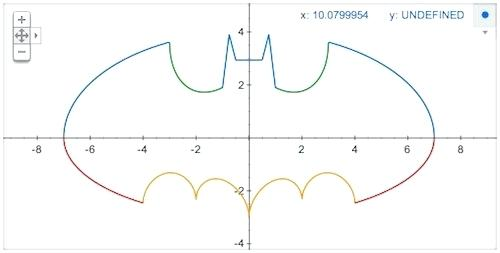
\includegraphics[width=0.8\linewidth]{batman.jpg}
    \caption{A cool graph. This image does not reflect the author's allegiance to the DC Comics universe.}
    \label{fig:1}
\end{figure}

\section{Example Section}
This is an example of a numbered section. Sections typically seen in a research paper are Related Work, Preliminaries, Data, Methodology, Experiments, Results and Discussion. The order in which these sections appear may depend on the venue.

\subsection{Example Subsection}
This is an example of a subsection. For example, Definitions could be a subsection of the Preliminaries section.

\section{Formulae, Tables}
\subsection{Typing Equations in \LaTeX}
This subsection demonstrates the use of inline formulae, like $e=mc^2$, or equations like the one below on a separate line. \[\int_a^b x^2\;\mathrm{d}x= \tfrac{1}{3} x^3 \Big|_a^b\]

For numbered equations, we use the \textit{equation} environment:

\begin{equation}
    \int_a^b x^2\;\mathrm{d}x= \tfrac{1}{3} x^3 \Big|_a^b
\end{equation}

\subsection{Tables}
This subsection demonstrates the use of tables in a \LaTeX document. Resources like \href{https://www.tablesgenerator.com/}{\emph{tablesgenerator.com}} can be used to generate code for tables like the one below.\

\begin{table}[h]
    \centering
    \begin{tabular}{ |p{3cm}||p{3cm}|p{3cm}|p{3cm}|  }
     \hline
     \multicolumn{4}{|c|}{Country List} \\
     \hline
     Country Name     or Area Name& ISO ALPHA 2 Code &ISO ALPHA 3 Code&ISO numeric Code\\
     \hline
     Afghanistan   & AF    &AFG&   004\\
     Aland Islands&   AX  & ALA   &248\\
     Albania &AL & ALB&  008\\
     Algeria    &DZ & DZA&  012\\
     American Samoa&   AS  & ASM&016\\
     Andorra& AD  & AND   &020\\
     Angola& AO  & AGO&024\\
     \hline
    \end{tabular}
    \caption{A Random Table}
    \label{tab:my_label}
\end{table}

References to books \cite{DUMMY:1} or articles \cite{ARTICLE:1} can be made like this, with the full citations defined in a \emph{.bib} file.

\bibliography{references}
\bibliographystyle{ieeetr}

\end{document}